\chapter{Felhasználói dokumentáció} % User guide
\label{ch:user}

Az alkalmazás készítése során fontos szempont volt, hogy egy felhasználóbarát webáruházat hozzak létre. A webshop használata egyszerű, letisztult felülettel rendelkező program olyan funkciókkal kiegészítve, amelyik megkönnyítik az átlagos vásárlók számára az oldal kezelését. A fejezet célja, hogy bemutassa az alkalmazás azon tulajdonságait, amelyek nem feltétlenül egyértelműek egy hétköznapi kliens számára, ezzel is elősegítve a webalkalmazás gördülékeny felhasználását.


\section{Alkalmazás indítása} % Enumerations and lists

Egy hétköznapi felhasználó számára talán ez a legnagyobb kihívás a program használatával kapcsolatban. Az alkalmazás indítására két módszer közül választhatunk, melyek a következőek:

\begin{compactenum}
	\item Megnyitni böngésző segítségével a weboldalt: \ref{section:browser} fejezet
	\item Megnyitni localhostról a projektet: \ref{section:localhost} fejezet
\end{compactenum}

\bigskip
Mindkettő technika részletes bemutatásra kerül a következő alfejezetekben.

\label{section:browser}
\subsection{Alkalmazás indítása böngészőből}
Az első és legkönnyebben alkalmazható stratégia, hogy valamilyen előre telepített webböngésző (Chrome, Firefox, Opera..stb.) segítségével megnyitjuk az Amazon AWS\cite{aws} szerverére telepített weboldalt. A felület ezen az URL-en érhető el: \url{http://webbeauty.us-east-2.elasticbeanstalk.com}

\label{section:localhost}
\subsection{Alkalmazás indítása saját gépről}
Az előző  módszert azért neveztem könnyebben alkalmazhatónak, mert ha saját gépről szeretnénk indítani az alkalmazást, nem csak le kell klónoznunk azt a GitHubról, hanem több különböző szoftvert kell telepítenünk, mielőtt el tudnánk indítani a projektet. A program fordításához szükségünk lesz a \textit{Node.js} szoftverrendszerre \cite{nodejs:online}. Továbbá elengedhetetlen a gépünkről az Angular CLI\cite{cli}. Ez egy parancssori interfész az Angular keretrendszerhez. A kód futtatásához szükségünk van rengeteg eszközre, amely lefordítja és optimalizálja a kódot, az Angular CLI ezt biztosítja a projekt számára. A kód fordításához szükségük lesz egy integrált fejlesztői környezetre (IDE). Én a Visual Studio Code\cite{vs:code} (VS Code) nyílt forráskódú kódszerkesztőjét használtam az alkalmazás elkészítése során, így ezt fogom bemutatni. A következő felsorolásban összefoglalom azokat a lépéseket, amelyek segítségével eljutunk a program saját gépről való indításáig. 

\begin{enumerate}
	\item\label{step:first} A Node.js oldaláról\cite{nodejs:online} töltsük le és telepítsük a számítógépre megfelelő .exe kiterjesztésű fájlt.
	\item Az általam felöltött és publikusan elérhető GitHub repository-t\cite{szakdolgozat2021} klónozzuk le az eszközünkre.
	\item Töltsük le és telepítsük a Visual Studio Code\cite{vs:code} nevezetű programot.
	\item Nyissuk meg a VS Code alkalmazást és telepítsük a következő bővítményeket: Angular Essentials, Material Icon Theme.
	\item A Visual Studio Code segítségével töltsük be a leklónozott projekt mappáját, és nyissunk meg egy új terminált.
	\item A terminálban lépjünk be a \textit{szakdolgozat} nevezetű mappába és futtassuk le a következő parancsot: \verb|npm install -g @angular/cli|
	\item Mivel az Angular CLI önmagában nem elegendő, futtassuk le a következő parancsot: \verb|npm i|. Ennek a parancsnak a segítségével letöltődik minden kiegészítő fájl, ami használatban van a programon belül.
	\item Mielőtt parancssor segítségével elindítanánk az alkalmazást be kell lépnünk a projekthez tartozó MongoDB\cite{mongo} adatbázisba. Itt hozzá kell adnunk a \textit{hálózati hozzáférés} nevezetű menüpont alatt a gépünk IP címét, különben nem tud csatlakozni a szerveroldalunk az adatbázishoz.
	\item A meglévő terminálunk mellé nyissunk meg egy újat, és futtassuk le az egyikben az \verb|npm run start|, a másikban az \verb|npm run start:server| parancsot. az utóbbi a kliensoldalt, míg az előbbi a szerveroldali kódokat futtatja és fordítja le.
	\item Ha sikeresen lefordult a kód, akkor a böngésző URL helyére a \textit{localhost:4200} címet begépelve láthatjuk a webáruház oldalát.
\end{enumerate}


\section{Alkalmazás kezelése}
Az alkalmazás felületét két részre bonthatjuk. Az alábbi \ref{fig.exemple-1}-es ábrán láthatjuk ezt a két rendszert, amiben a felhasználó, tulajdonos és az admin által elért funkciókat foglalja össze use case diagram segítségével. Az első rész maga a webáruház, amin a vásárlók megtekinthetik a termékeket és megrendelhetik őket, továbbá megnézhetik az üzemeltető által közzétett híreket, ezen felül különböző forrásokból információkat érhetnek el a vásárlással kapcsolatban. A második rész az üzemeltető által karbantartott adminisztrációs oldal. Ennek használatához hitelesítés szükséges, ezzel is védve a vásárlók és a webáruház adatait. Az admin felületen lehetőség van ezen adatok kezelésére, szerkesztésére.
\begin{figure}[H]
	\centering
	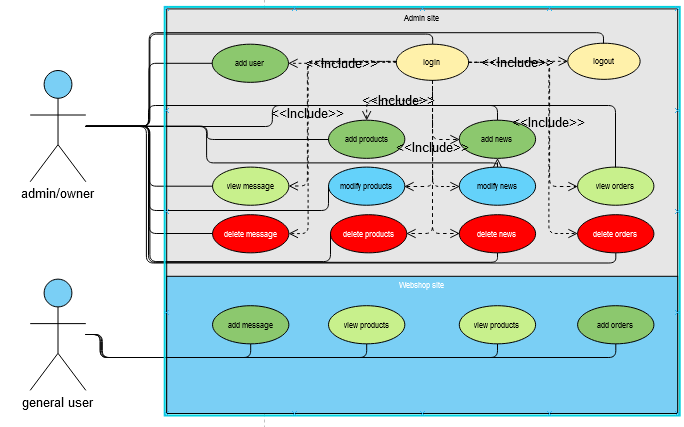
\includegraphics[width=1.0\textwidth]{images/use_case_diagram.PNG}
	\caption{Use case diagram - Alkalmazás funkciói}
	\label{fig.exemple-1}
\end{figure}

\subsection{Webshop felület kezelése}
A webáruház kezelése igen egyszerű az átlagos felhasználó számára. Számos funkcióval rendelkezik az alkalmazás, amelyek elősegítik, hogy egy letisztult, felhasználóbarát programot használjanak a vásárlók.
Az áruház szerkezeti felépítése három fő részből áll:
\begin{description}
	\item[Menüsor] vagy más néven \textit{toolbar}. A \ref{fig.exemple-2}-es ábrán a webáruház főoldalának egy részét láthatjuk. A kép tetején található az alkalmazás webshopjához tartozó vezérlőfelület, ami a programban \textit{toolbar} néven található meg. A vezérlőfelület bal oldalán láthatóak különböző menüpontok, amelyek segítségével navigálhatunk a különböző oldalak között. A jobb oldalán különböző funkciókkal bíró ikonokat és az oldal logóját láthatjuk. Az első ilyen ikon a nyelvválasztó, aminek a segítségével megváltoztathatjuk az oldal nyelvét. Jelenleg az angol és a magyar nyelv közül lehet választani. A mellette lévő bevásárlókocsit ábrázoló ikon segítségével érhető el a felület kosár funkciója, ami tartalmazza az eddig hozzáadott termékeket. A kosárban szereplő termékek számáról előzetes információt kaphatunk a felette lévő jelvény számból.
	
	\begin{figure}[H]
		\centering
		
\includegraphics[width=1.0\textwidth]{images/webshop_home.png}
		\caption{Az alkalmazás megjelenése}
		\label{fig.exemple-2}
	\end{figure}
	
	\item[A webáruház tartalma] (\textit{body}). Ez a menüsor alatt található meg, amit a fentebb kifejtett vezérlőfelület segítségével különböző oldalak tartalmi részét jeleníthetjük meg. Erre példákat \ref{fig.example-3}-as ábra a és b részén láthatunk.
	\begin{figure}[H]
		\centering
		\subcaptionbox{Termékek oldala}{
			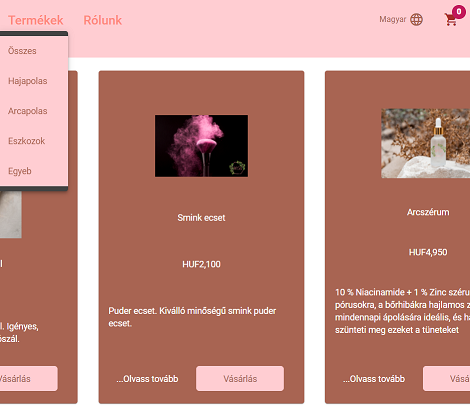
\includegraphics[width=0.45\textwidth]{images/products_page.png}}
		\hspace{5pt}
		\subcaptionbox{Hírek oldal}{
			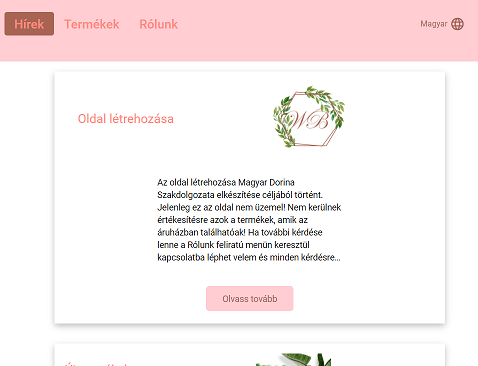
\includegraphics[width=0.45\textwidth]{images/news_page.png}}
		\caption{Webáruház tartalmi része}
		\label{fig.example-3}
	\end{figure}
	
	\item[Lábrész] (\textit{footer}). A \ref{fig.exemple-4}-es képen ez a felület látható. Itt olyan oldalak linkjei jelennek meg, amik tartalmazzák a vásárlókra és az oldalra vonatkozó fogyasztóvédelmi törvényeket és általános tájékoztatókat.
	\begin{figure}[H]
		\centering
		
\includegraphics[width=1.0\textwidth]{images/footer.png}
		\caption{Az oldal lábrésze}
		\label{fig.exemple-4}
	\end{figure}
	\item[A chatbot] funkció a \ref{fig.exemple-2}-es ábra legalján található \textit{Csevegjen velünk!} feliratú zöld gomb segítségével érhető el, aminek a bemutatását a \ref{section:shopping}-es Vásárlással kapcsolatos információk alfejezetben kívánok kifejteni.
	\item[Az alert üzenet] olyan információs felület, amik a felhasználó számára értesítést küld egy-egy feladat befejezésével kapcsolatban. Ilyen üzenetek lehetnek például, ha nem sikerül a betöltött űrlap feldolgozása, mint ahogy azt a \ref{fig.exemple-5}-ös ábrán is láthatjuk.
	\begin{figure}[H]
		\centering
		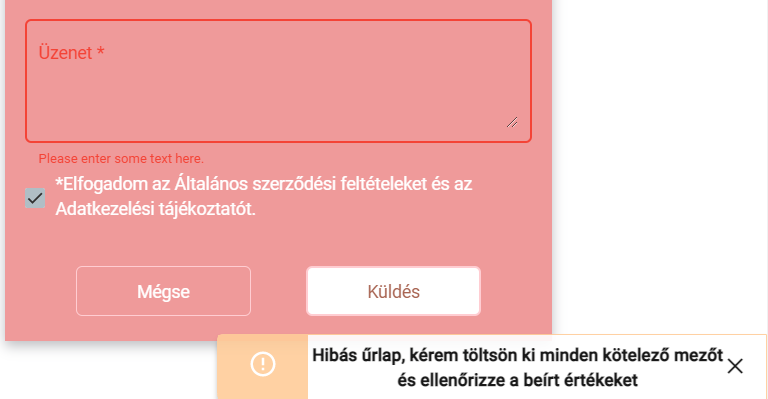
\includegraphics[width=1.0\textwidth]{images/alert_message.png}
		\caption{Alert üzenet}
		\label{fig.exemple-5}
	\end{figure}
\end{description}


\subsection{Adminisztrációs felület kezelése}
Az oldal eléréséhez szükség van a helyesen begépelt URL megadására a böngészőnkön keresztül, ami 

\begin{compactitem}
	\item localhost esetén: \url{http://localhost:4200/admin/login}
	\item AWS szerverre telepített weboldal esetén: \url{http://webeauty.us-east-2.elasticbeanstall.com/admin/login}
\end{compactitem}

Ha helytelenül gépeljük be a megadott webcímet, akkor az alkalmazás visszanavigál minket az oldal kezdőlapjára, viszont ha sikeresen begépeltük az adminisztrációs felület eléréséhez szükséges URL-t, akkor a \ref{fig.exemple-6}-os ábrán látott oldalt láthatjuk.
\begin{figure}[H]
	\centering
	
\includegraphics[width=1.0\textwidth]{images/bejelentkezes.png}
	\caption{Bejelentkezési oldal}
	\label{fig.exemple-6}
\end{figure}
Az adminisztrációs felület kezeléséhez szükségünk van az oldalt védő autentikáció feloldásához. Ez azt jelenti, hogy először be kell lépnünk a fejlesztő által megadott, vagy az üzemeltető által hozzáadott email cím és jelszó párossal az előbb említett címek valamelyikén. Sikeres bejelentkezéssel az oldal átnavigálásra kerül az admin felületre. Ez az oldal két fő részből áll: a vezérlési és a tartalmi részből.
\begin{description}
	\item[Vezérlési]rész, aminek segítségével megjeleníthetjük az alkalmazás tartalmi részét. A \ref{fig.exemple-7}-es képen ez a navigációs rész a bal oldalon található. Az admin felületen képesek vagyunk új termékeket vagy híreket hozzáadni, és a meglévőket lista formájában megtekinteni. Továbbá a fentebbiekben már említett kapcsolatfelvétel céljából a felhasználó által elküldött üzenetek is listázásra kerülnek az oldalon. Az alkalmazáson belül lehetőségünk van új felhasználói fiókot hozzáadni, viszont ezek a fiókok adatvédelmi okból nem megtekinthetőek és nem törölhetőek, csak adatbázis szinten. Ezen felül lehetőség van a bejelentkezett fiókot kijelentkeztetni, így visszalépve bejelentkezés hiányában nem tekinthetjük meg újból ezt a felületrészt.
	\begin{figure}[H]
		\centering
		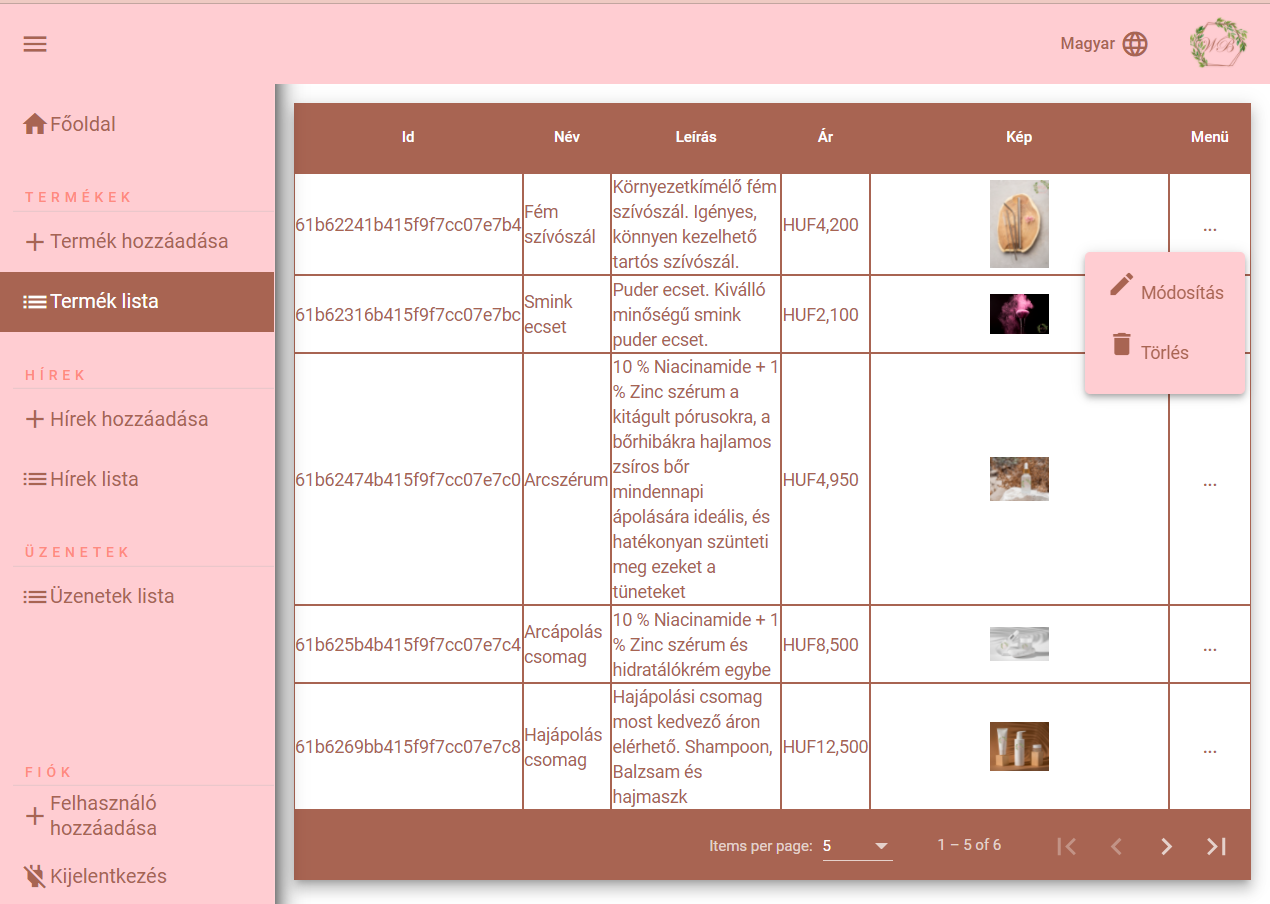
\includegraphics[width=1.0\textwidth]{images/admin.png}
		\caption{Adminisztrációs felület megjelenése}
		\label{fig.exemple-7}
	\end{figure}
	\item[A tartalmi rész] például a \ref{fig.exemple-7}-es ábra jobb oldalán látott táblázat, ami a  termékek listáját tartalmazza. Az oldal ezen részén lehetőségünk van az adatok módosítására, törlésére vagy a fentebb említett termék hozzáadására a megjelenő űrlap kitöltésével.
\end{description}

\section{Rendelési folyamat}
A rendelés folyamata hasonlóan zajlik, mint a legtöbb webáruházból való rendelés. A kiválasztott termékek bekerülnek a kosárba, majd a személyes adatok megadásával és a vásárlás befejezésével elküldésre kerül az oldal üzemeltetője számára, aki előkészíti azt. Az alábbi \ref{fig.exemple-8}-as kép pontosan ezt a folyamatot mutatja be szekvencia diagram segítségével.
\begin{figure}[H]
	\centering
	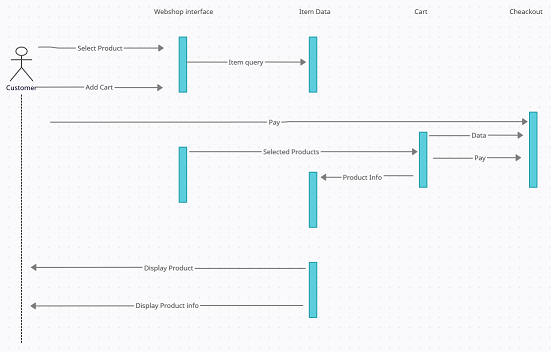
\includegraphics[width=1.0\textwidth]{images/szekvencia_diagram.PNG}
	\caption{Rendelési folyamat bemutatása - szekvencia diagram}
	\label{fig.exemple-8}
\end{figure}

A következő két alfejezetben bemutatom egy példán keresztül, hogyan is kerül egy rendelés leadása a termék kiválasztásától kezdve. Továbbá milyen feltételei és információ vonzatai van a webáruházon történő vásárlásnak.

\subsection{Rendelés leadása}
A rendelés leadásához először is szükséges, hogy legalább egy termék bekerüljön a bevásárlókosár tartalmába. Egy termék kosárba helyezésére két lehetőségünk van. Az első, ha a termékek listájánál a kiválasztott termék kártyáján a Vásárlás gombra kattintunk, mint ahogy a \ref{fig.exemple-9}-es ábrán is megfigyelhető.
\begin{figure}[H]
	\centering
	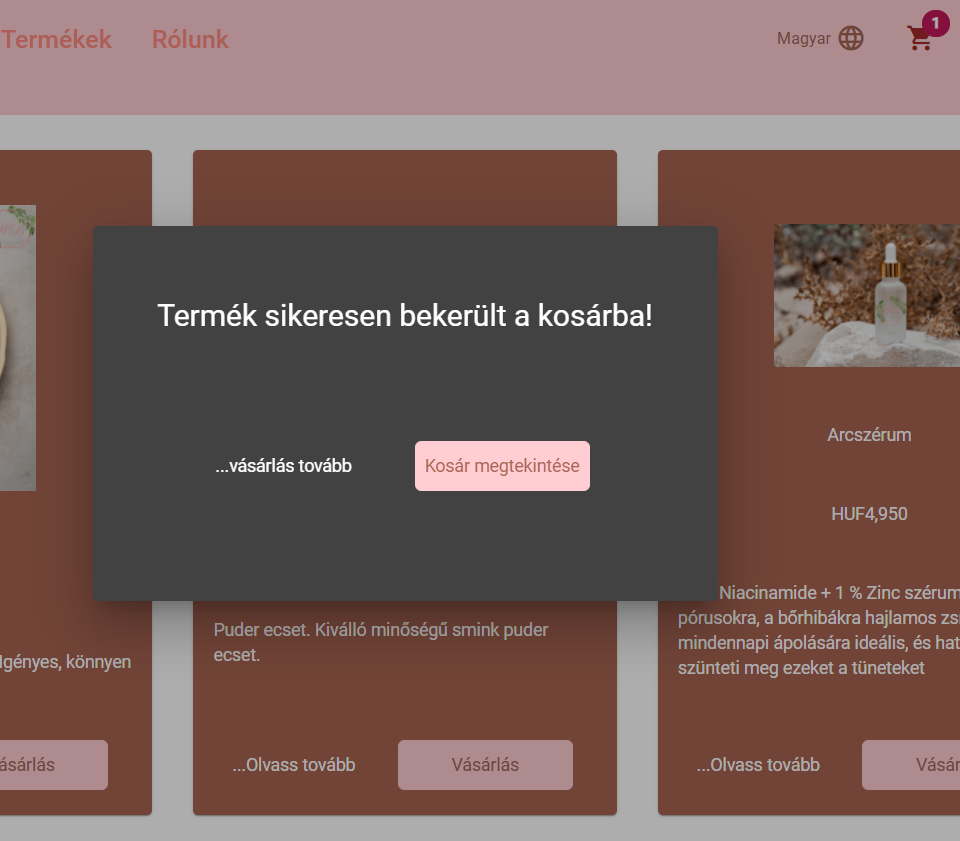
\includegraphics[width=1.0\textwidth]{images/termek_vasarlas_1.png}
	\caption{Termék vásárlása a termékek listáján keresztül}
	\label{fig.exemple-9}
\end{figure}

A második lehetőségünk az áru bevásárlókocsiba helyezésére, hogy a kiválasztott termék profil oldalán kattintunk a Vásárlás gombra. A különbség a két alternatíva között, hogy a második hozzáadás során megadhatjuk a kiválasztott áru mennyiségét, ahogy azt a \ref{fig.exemple-10}-es második kép példáján is láthatjuk.
\begin{figure}[H]
	\centering
	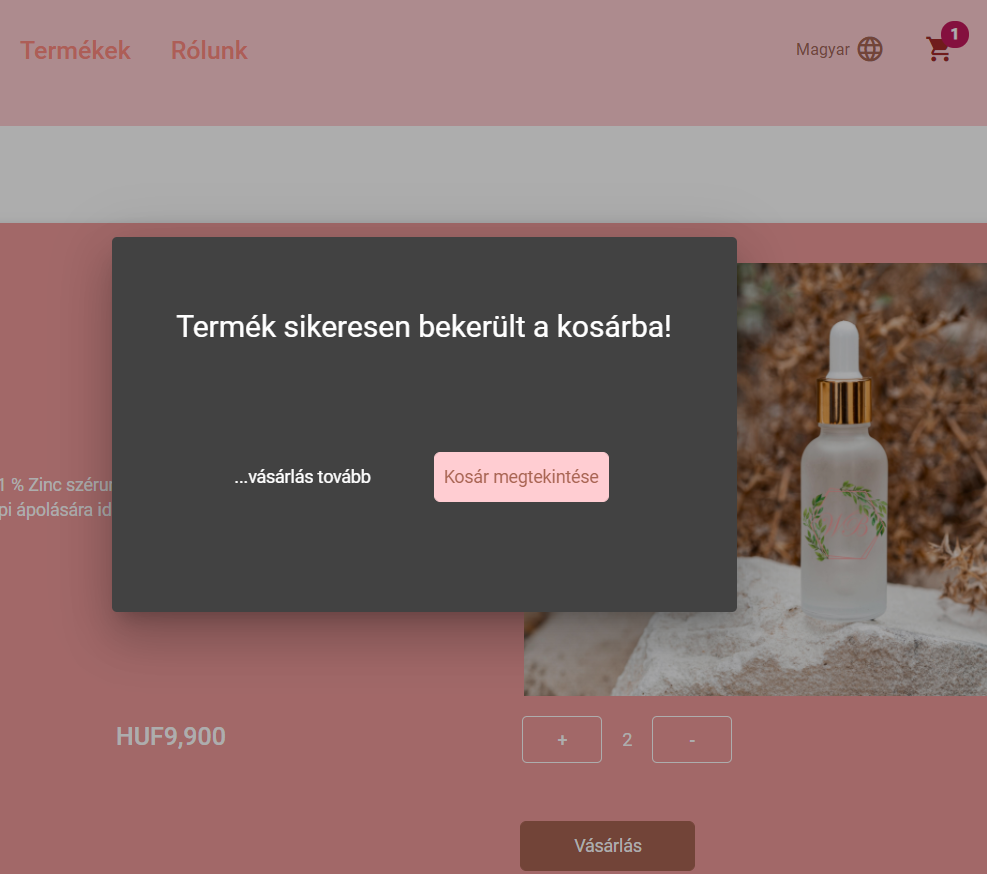
\includegraphics[width=1.0\textwidth]{images/termek_vasarlas_2.png}
	\caption{Termék vásárlása a termék profilján keresztül}
	\label{fig.exemple-10}
\end{figure}

Ha a kiválasztott termékek a kosárba kerültek, azokat megtekinthetjük úgy, ha a \ref{fig.exemple-9}-es és a \ref{fig.exemple-10}-es ábrákon is látott Kosár megtekintése gombot kiválasztjuk, vagy ha magára a bevásárlókocsi ikonjára kattintunk. Mindkettő lehetőség átirányít a kosár oldalára, ahol láthatjuk táblázat formájában a megvásárolandó árukat, mint azt a \ref{fig.exemple-11}-es képen is láthatjuk.
\begin{figure}[H]
	\centering
	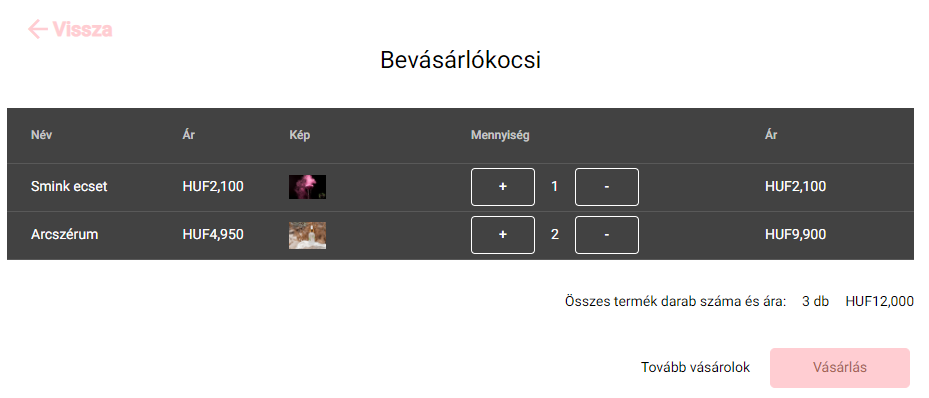
\includegraphics[width=1.0\textwidth]{images/kosar.png}
	\caption{Bevásárlókosár}
	\label{fig.exemple-11}
\end{figure}

A bevásárlókosár tartalmának módosításra lehetőségünk van a mennyiség oszlopában látható gombok segítségével. Ha csökkentjük vagy növeljük egy áru mennyiségét, akkor egyes adatok dinamikusan megváltoznak.

\bigskip
A táblázat alatti Vásárlás gombot kiválasztva az oldal átnavigál a fizetési felületre. A  \ref{fig.exemple-12}-es képeken látható, hogy ezen a felületen négy lépegető gomb található. Minden lépegetőnek külön funkciója van, amit a nevével azonosíthatunk.
\begin{figure}[H]
	\centering
	\subcaptionbox{Első lépegető gomb}{
		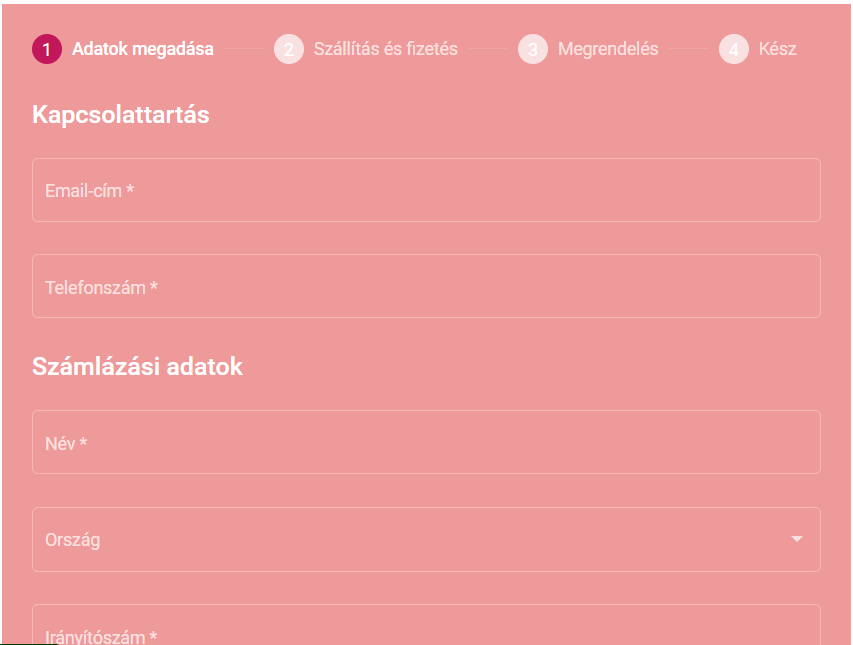
\includegraphics[width=0.45\textwidth]{images/fizetes_1.png}}
	\hspace{5pt}
	\subcaptionbox{Második lépegető gomb}{
		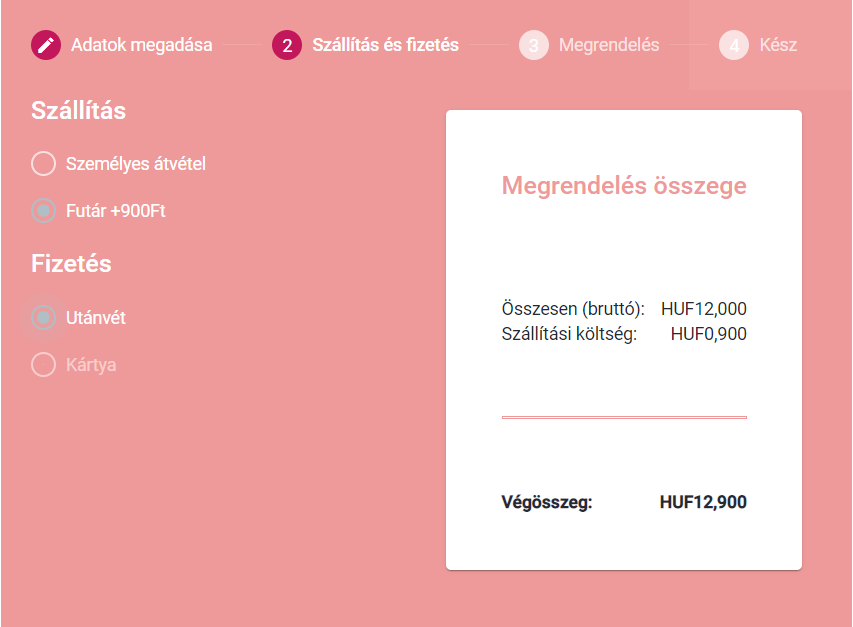
\includegraphics[width=0.45\textwidth]{images/fizetes_2.png}}
	\caption{Fizetési felület}
	\label{fig.exemple-12}
\end{figure}

Az első ilyen gombon adhatóak meg a szállítási és számlázási adatok űrlapon keresztül, aminek a helyes kitöltésével léphetünk a következő lépésre. A második lépegető gombon a szállítással és fizetéssel kapcsolatos információkat adhatjuk meg. A további lépegetőkön egy összefoglalót és visszajelzést kapunk a leadott rendeléssel kapcsolatban.

\label{section:shopping}
\subsection{Vásárlással kapcsolatos információk}
Az alkalmazáson belül számos információ rendelkezésre áll a vásárlók számára. A programban használt vásárlással kapcsolatos információforrások a következőek:

\begin{itemize}
	\item Chatbot: segítségével lehetőség nyílik a vásárlás során felmerülő kérdések feltevésére. Ezekre a kérdésekre a válaszadás dinamikus formában történik. Tekintsük meg az alábbi \ref{fig.exemple-13}-as ábrán illusztrált generált válaszadás folyamatát. A kép baloldalán látható, ahogy kiválasztjuk a feltevő kérdést és a kép jobb oldalán megválaszolásra kerül. Ha további kérdése van a vásárlónak a program megkéri, hogy forduljon az ügyfélszolgálathoz a megadott elérhetőségeken.
	\begin{figure}[H]
		\centering
		\subcaptionbox{Chat üzenet kérdések}{
			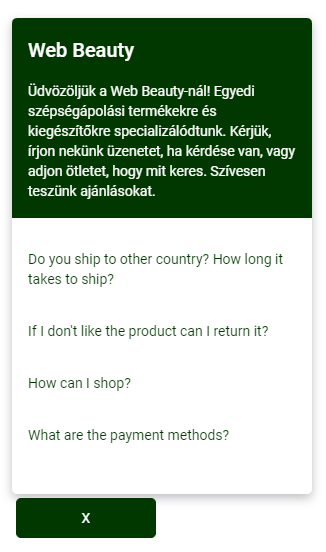
\includegraphics[width=0.45\textwidth]{images/chat_questions.png}}
		\hspace{5pt}
		\subcaptionbox{Chat üzenet válasz}{
			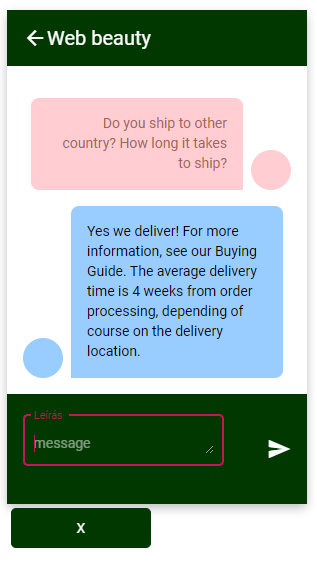
\includegraphics[width=0.45\textwidth]{images/chat_response.png}}
		\caption{Chat funció bemutatása}
		\label{fig.exemple-13}
	\end{figure}
	\item Általános Szerződési Feltételek minta: az Általános Szerződési Feltételek (rövidítve: ÁSZF) a vásárló és a szolgáltató közötti megállapodási szerződés. A szerződésbe foglalt két fél jogairól szól lényegében. Az oldalon található ÁSZF csak mintaként szolgál, mivel ennek megírása igen magas jogi ismereteket, akár jogász által elkészített dokumentumot igényel. Jelen esetben az oldalon található ÁSZF tartalma lementhető PDF formátumba. A \ref{fig.exemple-14}-es ábrán látott Letöltés PDF gombra kattintva az aszf.pdf kiterjesztésű fájl letöltésre kerül a gépünkre.
	\begin{figure}[H]
		\centering
		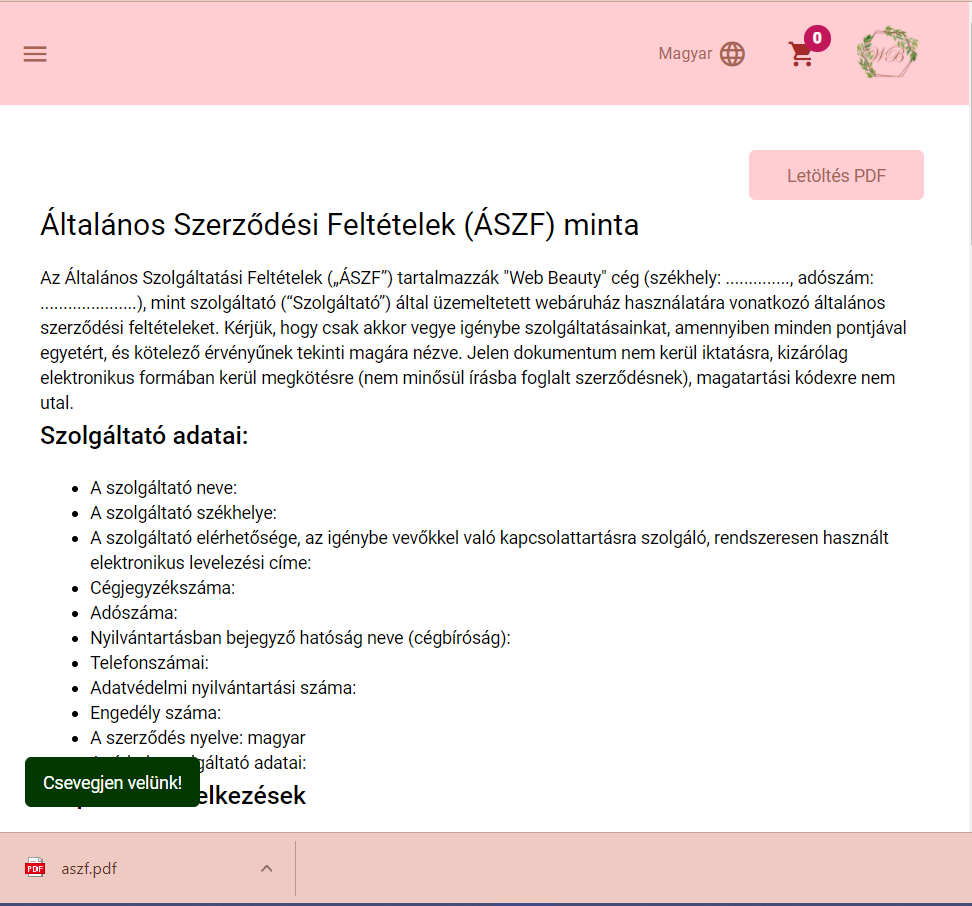
\includegraphics[width=1.0\textwidth]{images/pd_letoltes.PNG}
		\caption{ÁSZF letöltése}
		\label{fig.exemple-14}
	\end{figure}
	\item Adatkezelési tájékoztató: esetében az oldalon történő adatok tárolósáról szóló dokumentum. Az oldalon található adatkezelési tájékoztató ugyan úgy mintaként szolgál, mint az ÁSZF dokumentum. Erre is komoly jogszabályok vonatkoznak, aminek megírásához jogi tudás vagy egy jogász segítsége elengedhetetlen.
	\item Vásárlási útmutató: ez az oldal a vásárlás lépéseinek részletes leírására szolgál.
	\item Fizetési tájékoztató: az oldalon található vásárláskor igénybevehető szolgáltatások leírását tartalmazza, aminek segítségével információt szerezhet a vásárló a szállítással kapcsolatos díjazásokra és fizetési lehetőségekre.
\end{itemize}
